\documentclass[aspectratio=169]{beamer}

\usepackage{tikz}
\usetikzlibrary{shapes, backgrounds, arrows, positioning}
\usepackage{listings}
\usepackage[utf8,latin1]{inputenc}
\usepackage[style = apa, backend = biber, natbib = true]{biblatex}
\addbibresource{../../literature/lit.bib}

\makeatletter \def\newblock{\beamer@newblock} \makeatother  

\beamertemplatenavigationsymbolsempty
\setbeamertemplate{itemize items}[circle]
\setbeamertemplate{section in toc}[circle]
\mode<beamer>{\setbeamercolor{math text displayed}{fg=iwmgray}}
\setbeamercolor{block body}{bg=iwmorange!50!white}
\setbeamercolor{block title}{fg=white, bg=iwmorange}

% Definitions for biblatex
\setbeamercolor{bibliography entry note}{fg=iwmgray}
\setbeamercolor{bibliography entry author}{fg=iwmgray}
\setbeamertemplate{bibliography item}{}

\definecolor{iwmorange}{RGB}{255,105,0}
\definecolor{iwmgray}{RGB}{67,79,79}
\definecolor{iwmblue}{RGB}{60,180,220}
\definecolor{iwmgreen}{RGB}{145,200,110}
\definecolor{iwmpurple}{RGB}{120,0,75}

\setbeamercolor{title}{fg=iwmorange}
\setbeamercolor{frametitle}{fg=iwmorange}
\setbeamercolor{structure}{fg=iwmorange}
\setbeamercolor{normal text}{fg=iwmgray}
\setbeamercolor{author}{fg=iwmgray}
\setbeamercolor{date}{fg=iwmgray}

\title{Longitudinal data}
\author{Nora Wickelmaier}

\date{Last modified: \today}

\newcommand{\vect}[1]{\mathbf{#1}}
\newcommand{\mat}[1]{\mathbf{#1}}
\newcommand{\gvect}[1]{\boldsymbol{#1}}
\newcommand{\gmat}[1]{\boldsymbol{#1}}

\lstset{language = R,%
  basicstyle = \ttfamily\color{iwmgray},
  frame = single,
  rulecolor = \color{iwmgray},
  commentstyle = \slshape\color{iwmgreen},
  keywordstyle = \bfseries\color{iwmgray},
  identifierstyle = \color{iwmpurple},
  stringstyle = \color{iwmblue},
  numbers = none,%left,numberstyle = \tiny,
  basewidth = {.5em, .4em},
  showstringspaces = false,
  emphstyle = \color{red!50!white}}

\pgfmathdeclarefunction{gauss}{2}{%
  \pgfmathparse{1/(#2*sqrt(2*pi))*exp(-((x-#1)^2)/(2*#2^2))}%
}

\AtBeginSection[]{
  \frame{
    \tableofcontents[sectionstyle=show/hide, subsectionstyle=show/show/hide]}}

\setbeamertemplate{headline}{
 \begin{beamercolorbox}{section in head}
   \vskip5pt\insertsectionnavigationhorizontal{\paperwidth}{}{}\vskip2pt
 \end{beamercolorbox}
}

\setbeamertemplate{footline}{\vskip-2pt\hfill\insertframenumber$\;$\vskip2pt}

\begin{document}

\begin{frame}{}
\thispagestyle{empty}
\titlepage
\end{frame}

% \begin{frame}{Outline}
% \tableofcontents
% \end{frame}


\begin{frame}{Example: Growth curve model}
This example from linguistics is taken from \citet{Winter2016}\\[2ex]
\begin{itemize}
  \item Participants play a game of `vocal charades'
  \item At each round, a participant has to vocalize a meaning to the
  partner (e.g., `ugly') without using language (e.g., through grunting or
  hissing)
  \item The partner has to guess the meaning of the vocalization
  \item This game is played repeatedly with the finding that over time, a
  dyad converges on a set of nonlinguistic vocalizations that assure a high
  degree of intelligibility between the two participants in the dyad
\end{itemize}
\end{frame}


\begin{frame}{Example: Growth curve model}
\begin{itemize}
  \item Initially, participants may be struggling with the task and explore
  very different kinds of vocalizations
  \item Over time, they may converge on a more stable set of iconic
  vocalizations, that is vocalizations that resemble the intended referent
  (e.g., a high-pitched sound for `attractive' and a low-pitched sound for
  `ugly')
  \item Finally, after even more time, the dyad may conventionalize to
  idiosyncratic patterns that deviate from iconicity and become
  increasingly arbitrary
\end{itemize}
\end{frame}

\begin{frame}[fragile]{Example: Growth curve model}
100 observations of three variables (simulated data set)\\[2ex]
  \begin{tabular}{lp{8cm}}
      Variable & Description \\
    \hline
      \texttt{dyad} & different pairs of subjects playing the vocal charades game\\
      \texttt{t} & sequential rounds for which the vocal charades game was played \\
      \texttt{iconicity} & iconicity measure \\
     \hline
  \end{tabular}

  \vspace{1cm}
  For better interpretation, \texttt{t} will be centered
  \begin{lstlisting}
dat$t_c <- dat$t - mean(dat$t)
  \end{lstlisting}
\end{frame}

\begin{frame}[fragile]{Visualization of data}
  \begin{columns}
    \begin{column}{.5\textwidth}
      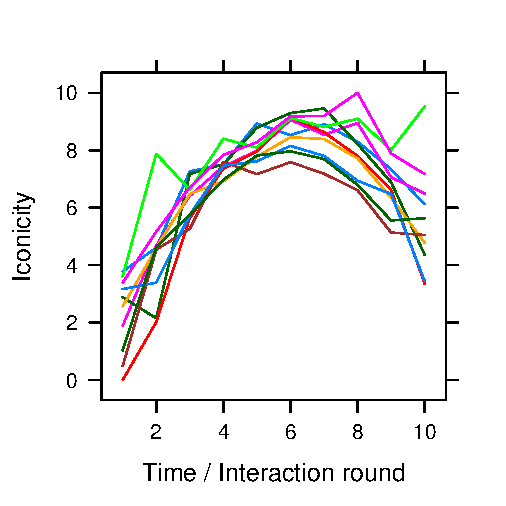
\includegraphics[scale=.8]{../figures/icon}
    \end{column}
    \begin{column}{.5\textwidth}
      \begin{lstlisting}
xyplot(
  iconicity ~ t, dat,
  groups = dyad,
  type = "l",
  xlab = "Time/Interaction round",
  ylab = "Iconicity")
      \end{lstlisting}
    \end{column}
  \end{columns}
\end{frame}

\begin{frame}[fragile]{Mixed-effects model with quadratic trend}
  We will now consider a model with uncorrelated random effects
  \[
    y_{ij} = \beta_0 + \beta_1 t_{ij} + \beta_2 t^2_{ij} + \upsilon_{0i} +
    \upsilon_{1i} t_{ij} + \upsilon_{2i} t^2_{ij} + \varepsilon_{ij}
  \]
with
\begin{align*}
  \begin{pmatrix}
    \upsilon_{0i}\\
    \upsilon_{1i}\\
    \upsilon_{2i}
  \end{pmatrix} &\sim
  N \left(\begin{pmatrix}
      0\\ 0\\ 0
  \end{pmatrix}, \,
  \begin{pmatrix}
    \sigma^2_{\upsilon_0} & 0 & 0\\
    0 & \sigma^2_{\upsilon_1} & 0\\
    0 & 0 & \sigma^2_{\upsilon_2}\\
      \end{pmatrix} \right)
    \text{ i.i.d.} \\
  \gvect{\varepsilon}_i &\sim N(\vect{0}, \, \sigma^2 \mat{I}_{n_i})
    \text{ i.i.d.}
\end{align*}
%\vspace{1cm}
  This model is fitted by
\begin{lstlisting}
gcm1 <- lmer(iconicity ~ t_c + I(t_c^2) +
  (1 | dyad) + (0 + t_c | dyad) + (0 + I(t_c^2) | dyad),
  data=dat, REML=F)
\end{lstlisting}
\end{frame}

\begin{frame}[fragile]{Visualization of model predictions}
  \begin{columns}
    \begin{column}{.5\textwidth}
      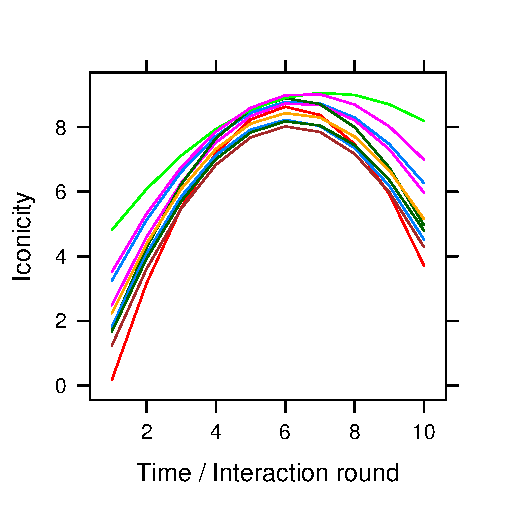
\includegraphics[scale=.8]{../figures/icon-pre}
    \end{column}
    \begin{column}{.5\textwidth}
      \begin{lstlisting}
xyplot(
  predict(gcm1) ~ t, dat,
  groups = dyad,
  type = "l",
  xlab = "Time/Interaction round",
  ylab = "Iconicity")
      \end{lstlisting}
    \end{column}
  \end{columns}
\end{frame}

\begin{frame}[fragile]{ML estimates of parameters}
\begin{lstlisting}
...
Random effects:
 Groups   Name        Variance Std.Dev.
 dyad     (Intercept) 0.152845 0.39095 
 dyad.1   t_c         0.002595 0.05094 
 dyad.2   I(t_c^2)    0.003504 0.05920 
 Residual             0.429691 0.65551 
Number of obs: 100, groups:  dyad, 10

Fixed effects:
            Estimate Std. Error t value
(Intercept)  8.45761    0.15849   53.36
t_c          0.35475    0.02793   12.70
I(t_c^2)    -0.22558    0.02078  -10.86
...
\end{lstlisting}
\end{frame}

\begin{frame}{Interpretation of results}
\begin{itemize}
  \item There are now two slopes, one for the effect of linear time ($t_c$,
  $\beta_1 = 0.35$) and one for the effect of quadratic time ($t_c^2$,
  $\beta_2 = -0.23$), both of which are allowed to differ by dyad
  ($\sigma_{\upsilon_{1i}} = 0.05$ and $\sigma_{\upsilon_{2i}} = 0.06$)
  \item The negative value for the quadratic term indicates the inverse
  U-shape
  \item The point of reversal is $t = \bar t + \frac{-\hat\beta_1}{2*\hat\beta_2} =
  5.5 + \frac{-.35}{2*(-.22)} = 6.29$ \item The model assumes that the
  random intercept and slopes are all
  uncorrelated
\end{itemize}
\end{frame}

\begin{frame}{Plots from the article}
\begin{center}
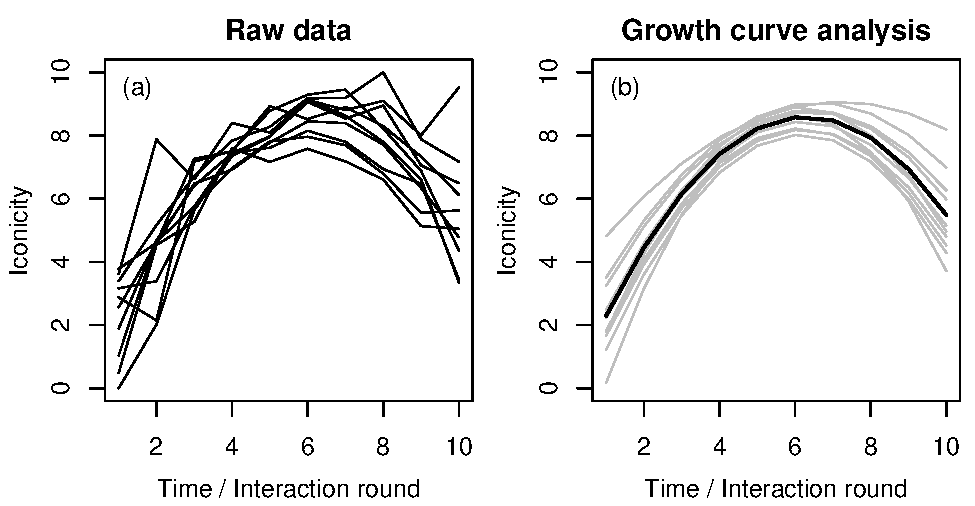
\includegraphics[scale=.66]{../figures/icon-both}
\end{center}
\end{frame}

% \begin{frame}[fragile]{}
%   \begin{lstlisting}
%   ##
%   \end{lstlisting}
% \end{frame}
% 
% }
% 
% \begin{frame}[fragile]{}
%   \begin{block}{Exercise}
%     \begin{itemize}
%       \item 
%     \end{itemize}
%   \end{block}
% \end{frame}

\appendix

%\begin{frame}[allowframebreaks]{References}
\begin{frame}{References}
%\renewcommand{\bibfont}{\footnotesize}
  \printbibliography
  \vfill
\end{frame}
 
\end{document}

